\documentclass[runningheads]{llncs}

\linespread{1.1}

\usepackage{lmodern}
\usepackage[english]{babel}

\usepackage{fontspec}

\raggedbottom

\usepackage{multicol}

\usepackage{float}
\usepackage{graphicx}
\graphicspath{{assets/}}
\usepackage{listings}

\PassOptionsToPackage{hyphens}{url}
\usepackage{hyperref}
\usepackage{cleveref}
\usepackage{nameref}

\usepackage[
  style   = numeric,
  sorting = none,
]{biblatex}
\bibliography{paper}

\newcommand{\german}[1]{{#1}}

\begin{document}

\title{Analysis of the \texorpdfstring{\\}{} Information Security Job Landscape \texorpdfstring{\\}{} in Austria}

\author{Markus Reiter}

\institute{University of Innsbruck, Austria}

\maketitle

\vspace{8em}

\begin{abstract}

In this paper we present a survey conducted by scraping and analysing various job search websites in order to get an overview of the current situation and trends regarding the information security job landscape in Austria.

\keywords{Information Security \and Scraping \and Job Advertisements}

\end{abstract}

\newpage

\section{Introduction}
\label{sec:introduction}

Information security management is more and more becoming an essential area of expertise for large and small companies alike. In order to get a better understanding of what the information security job landscape looks like in Austria, we conducted a survey of three job search websites popular in Austria: \textit{Monster}~\cite{monster}, \textit{Indeed}~\cite{indeed} and \textit{StepStone}~\cite{stepstone}. Our survey is comprised of three main steps: Firstly, we needed to scrape data each of the three job search websites. As will be explained in more detail in \autoref{sec:evaluation_of_scraping_tools}, we evaluated various scraping tools before we advanced to the actual implementation of the scraping process which will be explained in \autoref{sec:implementation}. The second part of our survey was then to use natural language processing in order to generate a more or less structured version of the information contained in the mostly unstructured text of the job advertisements. Lastly, we analysed and visualised the output data from the natural language processing step in order to fulfil our objective of forming a good overall perspective of the cybersecurity job landscape in Austria. In \autoref{sec:findings} we will present the findings we made during this process.

\section{Evaluation of Scraping Tools}
\label{sec:evaluation_of_scraping_tools}

The first step towards being able to analyse job advertisements on the internet is being able to properly retrieve them. For this reason, we evaluated various online scraping services.

The first contender we found was \textit{OctoParse} \cite{octoparse}, which provides a desktop application for scraping. Its free tier allows scraping unlimited pages on unlimited computers, with two concurrent scraping jobs. It allows configuring 10 different crawler configurations. There was, however, one major drawback to using \textit{OctoParse}: Its slogan claims “Easy Web Scraping for Anyone” – “Anyone” in this context meaning anyone with a Windows computer, since the desktop application is only supported on Windows. Linux and macOS users would have to run a virtual machine in order to use it, which is definitely not a viable solution for scraping a few websites. So we began looking for alternatives.

One alternative we found was \textit{ScrapingBot} \cite{scrapingbot}. Unlike \textit{OctoParse}, which provides a desktop application, \textit{ScrapingBot} does not provide an application at all. It is meant to be used similarly to using a proxy server. You can make an HTTP request with the same URL you normally would, and it responds with the contents, which includes any rendered JavaScript. Its free plan includes 100 API calls per month, therefore this also was no viable solution either, since the API calls would probably have been used up before the scraper was even working properly.

The next service we found was \textit{ScrapeStorm} \cite{scrapestorm}, which is very similar to \textit{OctoParse} in terms of what it provides. It offers a desktop application which works on Linux, macOS as well as Windows. In that regard, it was already looking like a better solution \textit{OctoParse}. The free plan allows 10 different crawler configurations and 1 concurrent local run. It also allows 100 exported rows per day, either into a file or directly into a database. All in all, \textit{ScrapeStorm} seemed like a good fit.

After choosing \textit{ScrapeStorm}, we started by setting up the crawlers. The websites we wanted to scrape are \texttt{monster.at}~\cite{monster}, \texttt{at.indeed.com}~\cite{indeed} and \\ \texttt{stepstone.at}~\cite{stepstone}.

For each website, we would have to implement two steps. First, we need to scrape the list of search results, which provides us with a list of links to the detail pages for the job advertisements. The second step is then to scrape the detail page itself.

As a first step, we tried scraping a detail page for a single job advertisement on \texttt{monster.at}. And it was a good thing we did, since it immediately highlighted a major problem. A job detail page on \texttt{monster.at} always includes the actual content of the advertisement inside of a nested \texttt{iframe} element. Using \textit{ScrapeStorm}, we were able to select that \texttt{iframe} element, but we failed to extract any data or text from it. The only thing we got was an empty string. This meant that we had to abandon the idea of using \textit{ScrapeStorm} for our purposes.

With this setback, we now had to find another way to scrape this data. After taking a second look at the \textit{ScrapingBot} homepage, we saw that it is using headless \textit{Chrome} for its back-end. We decided to venture further into this direction and found \textit{Selenium} \cite{selenium}, which can be used to programmatically use a web browser.

\textit{Selenium} supports all of the major web browsers, the only thing you need is the so called “webdriver” for the corresponding browser. Additionally, \textit{Selenium} can be used with a wide array of programming languages. For our purposes we chose to go with the Ruby version of \textit{Selenium}. Specifically, we chose to use \textit{Rake} \cite{rake}, which is similar to \textit{Make}, since it allows us to use the full functionality of \textit{Ruby} \cite{ruby} and specify tasks for each website. These scraping tasks can then be run with a simple \texttt{rake} command.

Given the setback we encountered on \texttt{monster.at}, the first thing we tried with \textit{Selenium} was to implement a simple task to extract the contents of the nested \texttt{iframe} element in their detail page layout. The first thing we needed to do was to fetch a job page. Next up, we needed to locate the nested \texttt{iframe} element; luckily this element is marked by a unique \texttt{id} field called \texttt{JobPreviewSandbox}. Once we had saved the nested \texttt{iframe} into a variable, we could use the \texttt{switch\_to} function provided by \textit{Selenium} to change to it from the main frame.

\begin{lstlisting}[language=Ruby]
iframe = find_element(id: 'JobPreviewSandbox')
switch_to.frame(iframe)
\end{lstlisting}

Seeing this proof-of-concept task working, we finally settled on using \textit{Selenium} and \textit{Rake} together with the \textit{Firefox} web browser.

\section{Implementation}
\label{sec:implementation}

\subsection{Scraping}
\label{sub:scraping}

As already briefly mentioned in \autoref{sec:evaluation_of_scraping_tools}, our goal was to implement scraping for \textit{Monster} (\href{https://www.monster.at/}{\texttt{monster.at}}), \textit{Indeed} (\href{https://at.indeed.com/}{\texttt{at.indeed.com}}) and \textit{StepStone} (\href{https://www.stepstone.at/}{\texttt{stepstone.at}}). In this section we will go into more detail about the exact steps which were necessary to reliably scrape each respective website.

\subsubsection{Monster}
\label{subsub:monster}

The first thing we needed to determine for \textit{Monster} \cite{monster} was how to perform searches. For this, we simply made a search request manually in a web browser. With the search string “information security” immediately noticed that it was escaped as \texttt{information-security} rather than the standard way to escape HTML, i.e. \texttt{information\%20security}. We needed to consider this when building the query URL.

Next up, we needed to assess how search results are paginated. \textit{Monster} does not use a classic pagination method using query string parameters, but rather uses a single “infinite” list which loads new search results automatically when you scroll to the bottom, or alternatively, click the “load more jobs” button.

With \textit{Selenium}, it was quite easy to extract all URLs leading to detail pages from the result list. Loading more than the first “page” of results was, however, quite convoluted. Simply scrolling down was not a good option, since then there would be no good way of knowing when to stop scrolling. Conveniently, \textit{Selenium} provides function to scroll to a given element, so we simply tried selecting the “load more jobs” button and scrolling to it. This is where we hit another problem. We could scroll the the button, but we were not able to click on it due to a pop-up blocking exactly the lower part of the page where the button is located, which meant we first had to dismiss this pop-up, which further meant introducing another potential point of failure, but for the moment, this solution was working.

In essence, the workflow for parsing URLs was as follows:

\begin{enumerate}
  \item Perform search request.
  \item Locate pop-up and dismiss it.
  \item Locate “load more jobs” button.
  \item \label{monster_workflow_1_scroll_to_button}
    Scroll to “load more jobs” button if it exists, otherwise go to step \ref{monster_workflow_1_select_results}.
  \item \label{monster_workflow_1_click_button}
    Click “load more jobs” button.
  \item \label{monster_workflow_1_select_results}
    Select all result URLs and collect them into an array.
\end{enumerate}

This workflow seemed to work as expected, however, we later encountered spurious error between step \ref{monster_workflow_1_scroll_to_button} and \ref{monster_workflow_1_click_button}. As mentioned previously, new search results are automatically loaded when you scroll to the bottom of the page. Obviously, scrolling to the “load more jobs” button was triggering that functionality and render the reference to the button invalid, making step \ref{monster_workflow_1_click_button} fail. While searching for a solution, we came upon \textit{Selenium's} \texttt{execute\_script} function, which can be used to directly execute \textit{JavaScript} code in the current browser window. This function enabled us to directly click the “load more jobs” button without scrolling to it, which also made it possible to eliminate the step for locating and dismissing the pop-up.

The final workflow now looked like this:

\begin{enumerate}
  \item Perform search request.
  \item Locate “load more jobs” button.
  \item Click the “load more jobs” button if it exists, otherwise go to \ref{monster_workflow_2_select_results}.
  \item \label{monster_workflow_2_select_results}
    Select all result URLs and collect them into an array.
\end{enumerate}

For the second part, the detail page of the job advertisement, we could now loop through all URLs and extract information from each one. On \textit{Monster}, each detail page contains the job title and a subtitle. The subtitle usually contains the location of the open position. Additionally, there is a sidebar which contains further metadata like the contract type, category, career level and publication date. The main content of the job advertisement is embedded into a nested \texttt{iframe} element. As mentioned in \autoref{sec:evaluation_of_scraping_tools}, using \textit{Selenium}, we could easily extract the content of this \texttt{iframe} element using the \texttt{switch\_to} function. All other data we could extract equally easily by selecting the corresponding elements using CSS selectors.

\subsubsection{Indeed}
\label{subsub:indeed}

For \textit{Indeed} \cite{indeed}, the initial step to implement proper scraping was to implement fetching search results. Luckily, unlike on \textit{Monster}, the search string could be escaped as \texttt{information\%20security} using standardised HTML escape codes.

Pagination on \textit{Indeed} is using a query parameter called \texttt{start} which indicates the offset from the first result. Additionally, the pagination buttons are located at the bottom of the results page. With the “next page” button acting as the stop indicator we can trivially implement the gathering of all detail page URLs as described below:

\begin{enumerate}
  \item Initialise empty array.
  \item \label{indeed_workflow_1_search}
    Perform search request with offset \texttt{0}.
  \item Select all result URLs and add them to the array.
  \item If “next page” button exists, repeat step \ref{indeed_workflow_1_search} with offset + \texttt{10}.
\end{enumerate}

Similarly to \textit{Monster}, the detail pages on \textit{Indeed} contain the title of the job advertisement as well as a metadata section. Care has to be taken when extracting data from this metadata section, since not every detail page contains every entry. Most pages seem to contain the location, but only some contain the contract type of the open position. For this reason, we simply treat all of these as optional and ignore any \texttt{NoSuchElementError} when searching for the respective element. In contrast to \textit{Monster}, the main content of the advertisement is contained as plain text, so no special treatment is necessary in this case.

\subsubsection{StepStone}
\label{subsub:stepstone}

Implementing the gathering of search results on \textit{StepStone} \cite{stepstone} was largely similar to the workflow used for \textit{Indeed}. The search string can be escaped using the standardised HTML escape codes, furthermore there are some query parameters we make use of: The \texttt{fu} parameter can be used to set the job category. We used \texttt{1000000} for this parameter to specify the “IT \& Communications” category. For faster scraping, we also set the \texttt{li} parameter to \texttt{100} in order to display 100 results per page rather than the default 25. Finally, we use the \texttt{of} parameter to specify the result offset which is then used in the same way as for \texttt{Indeed}. \textit{StepStone} displays the pagination controls at the top of the results page. These include the current as well as the last page number. Using this information we can stop the loop once we reach the last page.

A detail page on \textit{StepStone} contains the job title at the top, followed by a metadata section. The metadata contains the location, type of contract and type of employment (i.e. full-time or part-time). The main content of the job advertisement, similarly to \textit{Indeed}, is a section containing plain text. This makes it trivial to extract all data.

\subsubsection{Storage of Scraped Data}
\label{subsub:storage_of_scraped_data}

Now that we had successfully built the foundation for properly scraping all websites, the last step was to store the scraped data in a format which can be used for further processing. Using a full-fledged database solution, e.g. MySQL or Postgres, was out of the question from the start. Setting up a dedicated database server for what is -- relatively speaking -- a very small amount of data would add too much maintenance overhead. Another aspect to consider is the data layout.
In database terms, we need to store only a single table of data, which was another reason why we decided against using a database for storing the collected data altogether. This included embedded databases like SQLite which consist of a single file and don't need a dedicated server and client. Ultimately we decided on storing each scraping result in a separate \textit{JSON} file. \textit{JSON} is heavily used for APIs on the web which means that virtually every programming language supports deserialising and serialising data in \textit{JSON} format. To avoid duplicates, we chose to save the files as \texttt{<website>-<id>.json} where \texttt{<website>} is the name of the website, i.e. \texttt{monster}, \texttt{indeed} or \texttt{stepstone}. For the \texttt{id} we calculate the SHA2 checksum of the URL.

For example, the scraped data from the URL \\
\texttt{https://at.indeed.com/rc/clk?jk=db6f5459c93e648c\&fccid=1272531993b\\16790\&vjs=3} would be saved as
\texttt{indeed-43da336235334055a25f32a55e7cd3431\\28905d782cd749349659ca3d3d38174.json}.

\subsubsection{Removal of Duplicates}
\label{subsub:removal_of_duplicates}

After a couple of scraping runs, we noticed that there were duplicate results. This happened for all three websites. These duplicates were either completely equal or had only minor differences in their HTML source code. Nevertheless, we needed to introduce a post-processing step after the scraping is finished. We implemented a new \textit{Rake} task called \texttt{deduplicate} which reads all results and sorts them by date. We then convert the results' title and HTML body content to plain text and group the results according to that. Finally, we can find all duplicates by selecting all results with more than one entry in the corresponding group and remove all but the latest one.

\subsection{Natural Language Processing}
\label{sub:natural_language_processing}

Once the scraping was done, we could focus on extracting information from the scraped data. For the purpose of data extraction, we chose Python. Like Ruby, Python is an interpreted and dynamically typed language, which makes it a good candidate for natural language processing since we can iterate over code changes very quickly. We chose Python over Ruby due to the vast amount of libraries and frameworks available dedicated to natural language processing, first and foremost the Natural Language Toolkit (NLTK), arguably one of the most widely used platforms for natural language processing. It contains a great variety of tools including classification, tokenisation, stemming, tagging, parsing and semantic reasoning. \cite{nltk}

\subsubsection{Data Cleaning}
\label{subsub:data_cleaning}

The first step when performing any sort of natural language processing should be data cleaning. Specifically, this means removing irrelevant data and bringing the data into a format that can be processed more easily than the raw source. In our the main part that needed to be cleaned was the body text of each result. Each result contains the raw HTML source code of the body text, so the first step was to strip the text from any contained HTML tags. We used the aptly named \texttt{html2text} Python package for this purpose. After further inspection of the results, we noticed that some contained formatting, links and images in Markdown format. We quickly realised that \texttt{html2text} is in fact an HTML to Markdown converter instead of a HTML to plain text converter as we previously deemed from the name. Luckily, \texttt{html2text} provides \texttt{ignore\_emphasis}, \texttt{ignore\_links} and \texttt{ignore\_images} options which can be used to remove the Markdown output for these elements. Once we had the plain text version of the body content, we could subsequently use the \texttt{word\_tokenise} function from the NLTK to split the text into tokens to make further processing easier.

\subsubsection{Extracting the Salary}
\label{subsub:extracting_the_salary}

The first data point we decided to extract was the salary for the advertised job. Even with only this single data point, there is a lot of variation in how the salary is represented.

\begin{figure}
	\centering

  \begin{multicols}{3}
    \begin{description}
      \item 43,595 Euros
      \item 30k Euros
      \item 3,100.00 EUR
      \item EUR 2.800,-
      \item EUR 50k
      \item EUR 5700
      \item EUR 2.600,00
      \item 70.000 €
      \item € 4.209,-
      \item € 3.933,0
      \item € 55.000,--
      \item € 65.000,---
      \item 65,000 €
      \item €60,000
      \item €85k
      \item €3.007,20
      \item 80.000 Euro
      \item 60000 €
    \end{description}
  \end{multicols}
  \caption{An incomplete list (extracted from actual data) of number formats used to represent salary.}
  \label{salary_formats}
\end{figure}

As seen in \autoref{salary_formats}, the diversity of number formats is quite extensive. To explain the steps we took to further clean the input data, we will define the \texttt{clean\_text} step as cleaning the complete text before it is tokenised and the \texttt{clean\_word} step as cleaning a single word after tokenisation.

The first step we took was to add another sub-step to our existing \texttt{clean\_text} step in which we used the regular expression \texttt{/(EUR|€)/} and replace it with \texttt{' \textbackslash1 '}, i.e. we add an extra space around \texttt{EUR} and \texttt{€} to cover the case where there is not already a space between the currency and the amount. We don't care about introducing extra spacing when there already is a space since the tokenisation will remove it anyways.

Now that we have ensured that the currency is separated from the amount, we can add another sub-step to \texttt{clean\_word}. Here we introduce a trivial replacement and replace all words which are equal to \texttt{'€'}, \texttt{'eur'}, \texttt{'euro'} or \texttt{'euros'} with \texttt{'€'}.

Next, we add another sub-step to \texttt{clean\_word} which removes any trailing \texttt{',-'} from numbers. We use a regular expression here to also catch cases with more than a single hyphen. Similarly to the trailing \texttt{',-'}, we replace a trailing \texttt{'k'} with \texttt{'000'}.

The only thing left to do now is to normalise the decimal format (i.e. \texttt{XXXXX,XX}, \texttt{XXXXX.XX}, \texttt{XX.XXX,XX}) \texttt{XX,XXX.XX}, to \texttt{XXXXX.XX} in order to be able parse it in a later step. For the normalisation, we assume that the salary amount has at most two decimal places. We use a regular expression to match 0-2 decimal places with any delimiter symbol and group everything else together. This gives use the integer part with all delimiter symbols and the decimal part as only numbers. Now we simply remove all delimiters from the integer part and combine both parts again with a \texttt{'.'}.

In order to eventually extract the salary, we loop through all cleaned tokens as 2-grams so we can match the currency symbol either before or after the number.

\subsubsection{Extracting the Type of Education}
\label{subsub:extracting_the_type_of_education}

Another data point we wanted to extract is the level of education required for a given job. We started by looking at some advertisements and then began building some patterns which we could use in our \texttt{guess\_education} function. Some obvious patterns include \texttt{<type>-Abschluss} and \texttt{<type>abschluss} with concrete examples being “\german{HAK-Abschluss}” and “\german{Pflichtschulabschluss}”. Since the \texttt{guess\_education} function receives the input as individual tokens, compound words including acronyms such as “\german{HTL-Abschluss}” would already be split into \texttt{'htl'} and \texttt{'abschluss'}. Given that there are only a handful of acronyms we decided for simplicity's sake to hardcode the most common ones: \texttt{'hak'}, \texttt{'hbla'}, \texttt{'htl'}, \texttt{'hlw'} and \texttt{'lfs'}. We grouped all of these into the \texttt{matura} category. Still, there were some patterns which fall into this category which were not yet recognised, such as “\german{Matura}” as a standalone term or “\german{Fachschulabschluss}”. For these, we simply check if any word contains these terms.

The next two obvious education types were the bachelor's and master's degree. For these, we again simply checked if any word contains the respective term and categorise them accordingly. Another related education type is an \german{FH} (\german{Fachhochschule}) degree which can be equivalent to either a bachelor's or master's degree. Here we again took the same approach as for the \texttt{matura} category, since both “\german{FH-Abschluss}” and “\german{Fachhochschulabschluss}” are commonly used terms.

With these types for higher levels of education covered, we could guess the education level only for less than half of the results. One type we missed previously was the completion of compulsory school. With compulsory school added to the list, we still were only detecting an education type for around half of all results. After inspecting some of the results which were still missing an education type, we found the two types which were still missing: completed apprenticeship (often referred to as “\german{abgeschlossene Ausbildung}”) and completed apprenticeship (often referred to as “\german{abgeschlossene Lehre}”).

With these two types the extraction rate was now at approximately 90\%. A few more results could be detected by extracting the words \texttt{'studium'} and \texttt{'universität'}/\texttt{'university'}, since some job advertisements refer to a bachelor's degree simply as “\german{abgeschlossenes Studium}” (completed studies) or list “\german{Universität}”/“University” as a requirement.


\subsubsection{Extracting the Type of Employment}
\label{subsub:extracting_the_type_of_employment}

We also wanted to know what type of employment a particular job advertisement pertains to, i.e. whether it is a full-time or part-time position and whether the contract is permanent or temporary. Some websites include this information in their metadata section, for others we would have to extract this data from the body text. Apart from the obvious keywords such as \texttt{'full-time'} and \texttt{'part-time'}, we also needed to look for the number of work hours per week in the body text, since some advertisements list the work hours explicitly instead of the more vague distinction between full-time and part-time. To extract this, we used a similar pattern to the one for extracting salaries: We loop through all pairs of words. If the first word is a number and the second word is either \texttt{'wochenstunden'} or \texttt{'hours'}, we parse the number. We assume \texttt{'full-time'} if that number is greater than 20, otherwise we assume \texttt{'part-time'}.

\subsubsection{Extracting the Location}
\label{subsub:extracting_the_location}

The next data point we needed to extract is the location of the job in question. Fortunately, all of the scraped websites include the location as a separate field in their respective metadata section. This way, we could limit our extraction to just this field. This field required a specialised data cleaning step which expands state acronyms. For example, we needed to replace \texttt{'W'} with \texttt{'Wien'} or \texttt{'Oö'} and \texttt{'OÖ'} with \texttt{'Oberösterreich'}. Additionally, we also replaced the English translations of states and used the German spelling as the canonical version.

Furthermore, we used a database containing all major cities in Austria \cite{austria_cities_database} in order to also catch cases where only the city is specified but the corresponding state is missing. With this database, we can then map the tokenised string to cities and states. In the end, we get a list of all extracted cities and another list of all extracted states. In case we are not able to extract anything from the metadata field, we fall back to running the same extraction function on the whole body text.

\subsubsection{Extracting of Certifications}
\label{subsub:extracting_of_certifications}

Up next was the extraction of certifications. We found an article listing the most prominent certifications of the year 2020 \cite{certifications}. Incidentally, the authors of this article also retrieved this list from performing a job board survey. Using the list of certifications mentioned in the article and a manual review of the scraped data, we came up with a list (as can be seen in \autoref{tab:certifications}) of all the certifications we wanted to extract.

\begin{table}[ht]
	\centering
  \caption{List of extracted certifications.}
  \label{tab:certifications}

  \begin{tabular}{|l|l|}
    \hline
    \textbf{Certification} & \textbf{Description}                                \\ \hline
    CEH                    & Certified Ethical Hacker                            \\ \hline
    CISA                   & Certified Information Security Auditor              \\ \hline
    CISM                   & Certified Information Security Manager              \\ \hline
    CISSP                  & Certified Information Systems Security Professional \\ \hline
    CRISC                  & Certified in Risk and Information Systems Control   \\ \hline
    ITIL                   & Information Technology Infrastructure Library       \\ \hline
    CIA                    & Certified Internal Auditor                          \\ \hline
    ISO/IEC 27001          & Information Technology Security Techniques          \\ \hline
    HITRUST                & HITRUST Compliance Certification                    \\ \hline
    COBIT                  & COBIT Certification                                 \\ \hline
    ISO/IEC 22301          & Business Continuity Management                      \\ \hline
    CGEIT                  & Certified in the Governance of Enterprise IT        \\ \hline
    GIAC                   & GIAC Cybersecurity Certification                    \\ \hline
  \end{tabular}
\end{table}

In comparison to the other extraction tasks, extracting certifications was straight-forward given this fixed list. There was, however, still one adjustment needed for the data cleaning step with regards to the ISO/IEC certifications since some of them only specified \texttt{'ISO'} while others specified \texttt{'ISO/IEC'}. A few of them were also missing white space between the acronym and the number, e.g. \texttt{'ISO27001'}. For this reason, we added another regular expression replacement to the data cleaning step which normalises all of these occurrences to the canonical \texttt{'ISO/IEC~\#\#\#\#\#'} form.

\subsection{Data Visualisation}
\label{sub:data_visualisation}

Once the data extraction was implemented, naturally we wanted to visualise the collected data in order to make it easier to reason about and draw conclusions. We chose to use \textit{Jupyter} \cite{jupyter} for this purpose. Specifically we used \textit{Jupyter~Notebook}, which is an interactive environment in which you can write code and visualise data at the same time. This makes it very useful when experimenting as you can immediately see the results and you can encapsulate code parts into different sections. This saves a lot of time since you do not need to run the whole project on every change but can test the changes for separate sections individually. \textit{Jupyter} is developed in \textit{Python} \cite{python} but also supports a lot of other programming languages. For our purposes we chose to stick with \textit{Python} since there are many great tools available with regards to data analysis and visualisation. To further reorganise the collected data we used the well-known \textit{pandas} \cite{pandas} data analysis and manipulation tool. For data visualisation, we decided to use \textit{Plotly} \cite{plotly}, an open source graphing library. With the power of \textit{Python} and \textit{pandas}, it was relatively straight-forward to convert the collected data into the representation expected by \textit{Plotly} to create graphs. And due to the fact that we were using \textit{Jupyter}, we could immediately see the generated graphs.

\section{Findings}
\label{sec:findings}

Before discussing the findings we made, we will provide a short overview of the amount of data we collected as well as the amount of data which was eventually incorporated to generate the results in this section.

% ls data | wc -l
% ls data | grep monster | wc -l
% ls data | grep indeed | wc -l
% ls data | grep stepstone | wc -l

In total, we scraped 1538 job advertisements from all three websites. These are composed of 993 from \textit{Monster}, 282 from \textit{Indeed} and 263 from \textit{StepStone}. These results were aggregated over a time span of about two months by rerunning the scraping tasks roughly once per week in order to scrape newly added job advertisements.

\begin{figure}[H]
	\centering
  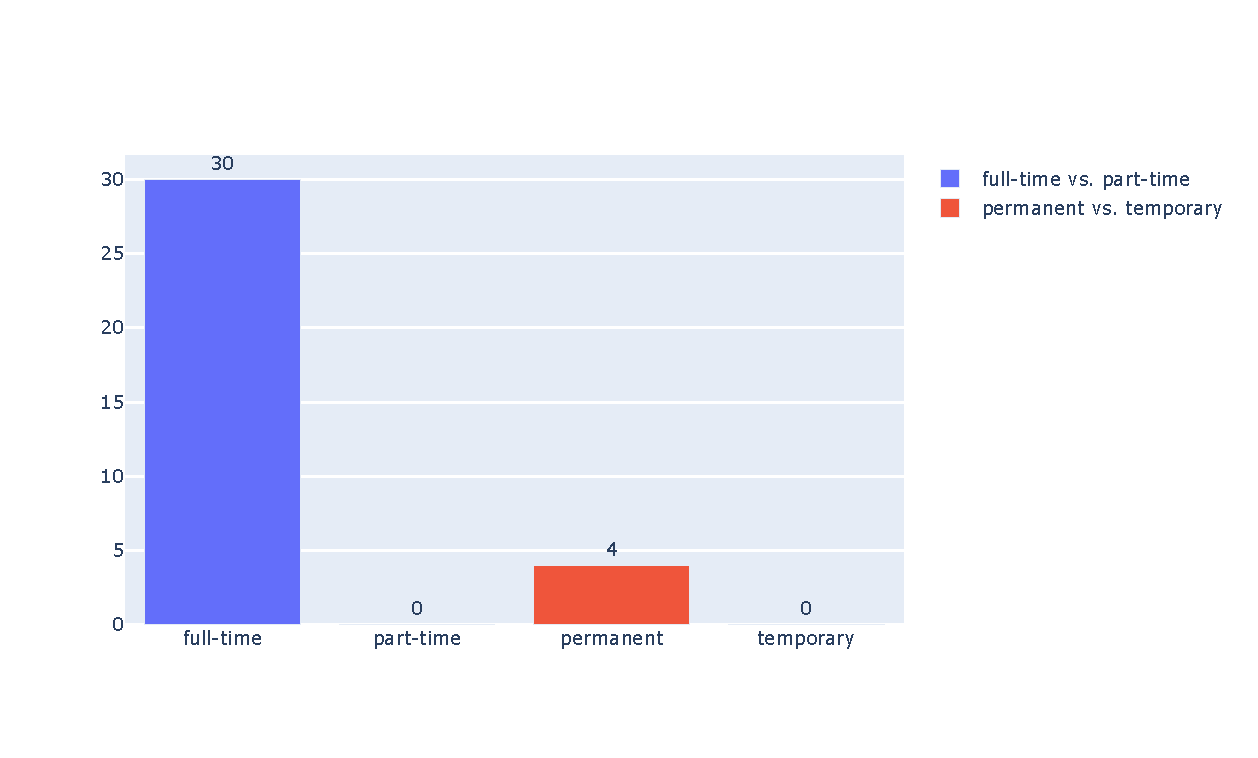
\includegraphics[width=\textwidth]{employment-type-bar-chart.pdf}
	\caption{Employment Type}
	\label{fig:employment_type_chart}
\end{figure}

After a review of the scraped data, we found that many advertised jobs had nothing to do with information security at all and were simply included as a consequence of the loose search algorithm provided by the job search websites. We therefore decided to add a final filter to the data depending to the job title. Once we added this filter we were left with 121 information security jobs out of 1538 total scraped jobs. All graphs presented in this section are based on this number.

Let us begin with the employment type. For the employment type we used two different distinctions: full-time vs. part-time positions and permanent vs. temporary positions.

In \autoref{fig:employment_type_chart} we can see that 95\% of cybersecurity jobs are listed as full-time positions and the remaining 5\% do not specify this information at all. The permanence of the position is even less common with only 3.3\% of permanent positions and the remaining 96.7\% leaving this information unspecified. In general, the assumption for leaving this information unspecified is a permanent full-time position, which means that at this point virtually all open cybersecurity positions are permanent full-time positions.

Next up we will take a look at the required level of education for information security jobs. As shown in \autoref{fig:education_chart}, the majority of positions -- around 59\% -- require a bachelor's degree while only around 9\% require a master's degree.

\begin{figure}[H]
	\centering
  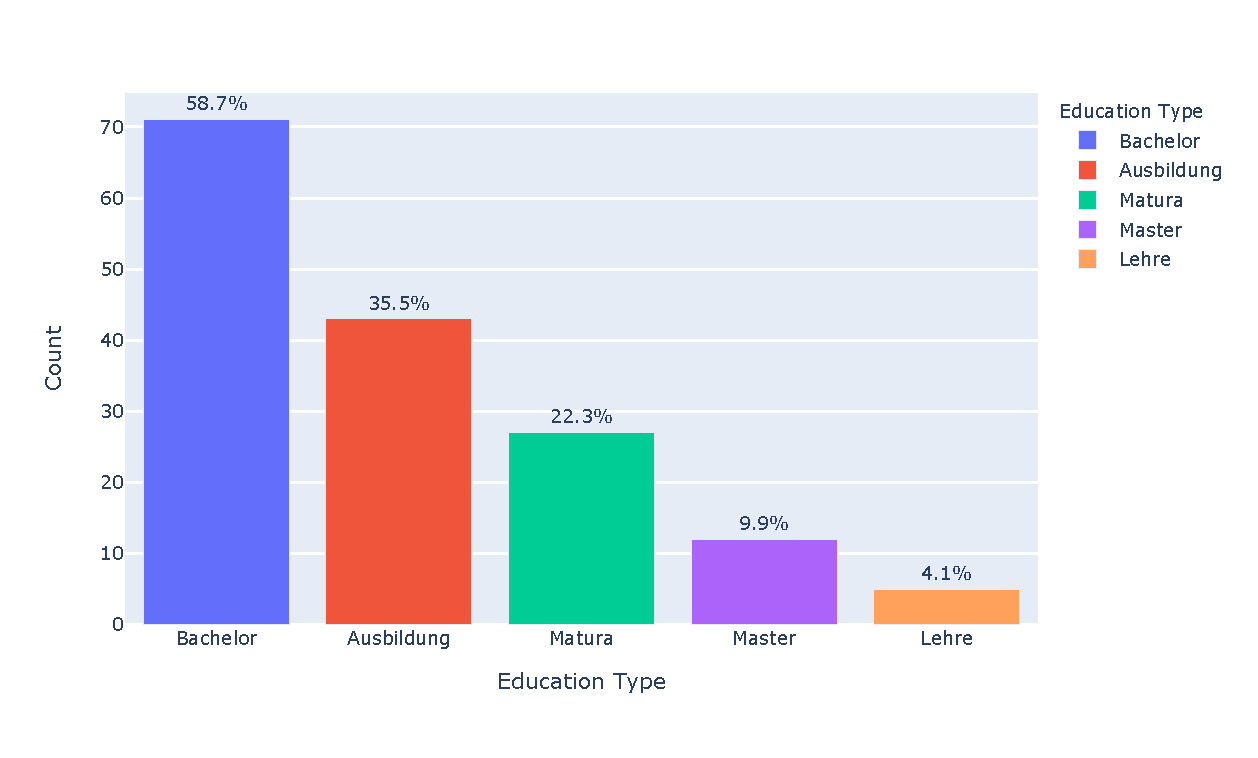
\includegraphics[width=\textwidth]{education-bar-chart.pdf}
	\caption{Education}
	\label{fig:education_chart}
\end{figure}

The second most common requirement is an apprenticeship (“\german{Ausbildung}”) at around 36\%, followed by the “\german{Matura}” with 22\%. After a manual review of the 4\% belonging to apprenticeship (“\german{Lehre}”), these seem to be mostly false positives, at least in our case when only taking information security jobs into account. The false positives in this case are due to the fact the the term “\german{Lehre}” is not only used to describe an apprenticeship but also teaching -- also referred to as “\german{Lehre}” -- positions.

\begin{figure}[H]
	\centering
  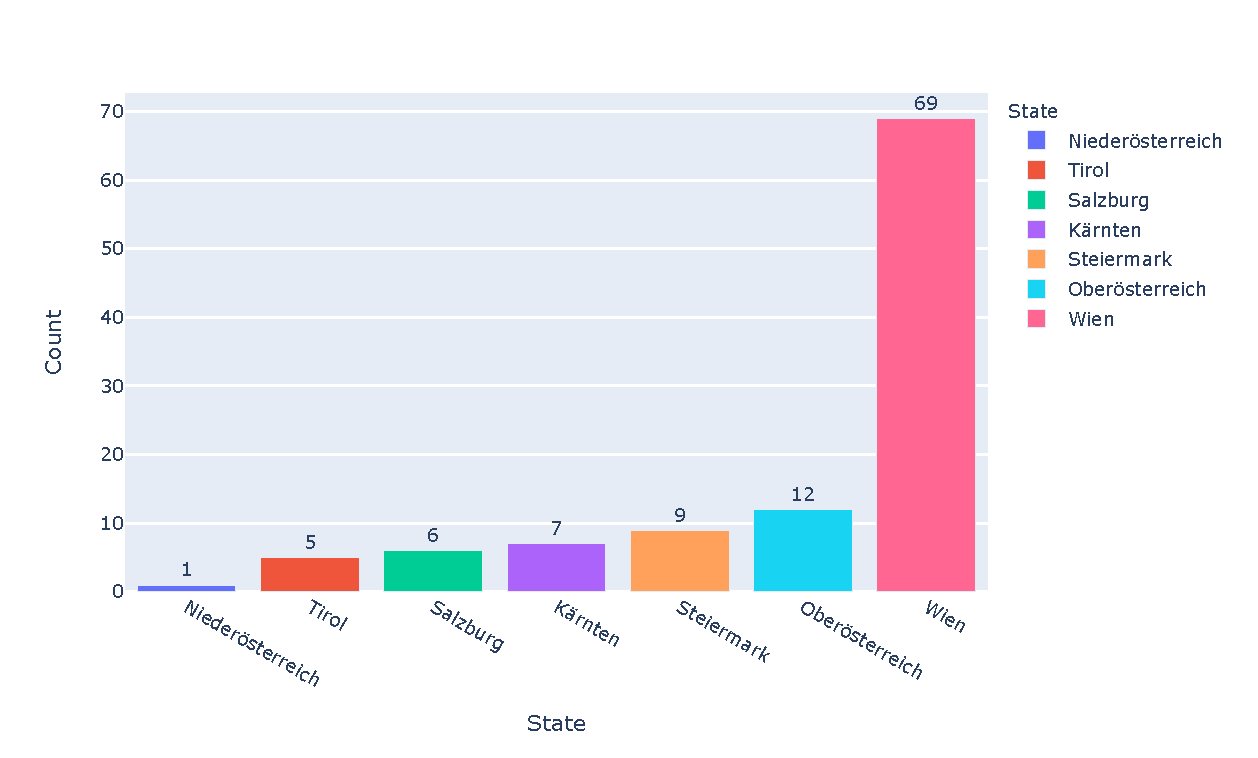
\includegraphics[width=\textwidth]{location-bar-chart.pdf}
	\caption{Location}
	\label{fig:location_chart}
\end{figure}

The distribution across the states of Austria was another point we wanted to analyse. The vast majority of advertisements are for positions in Vienna at about 57\%.

\begin{figure}[H]
	\centering
  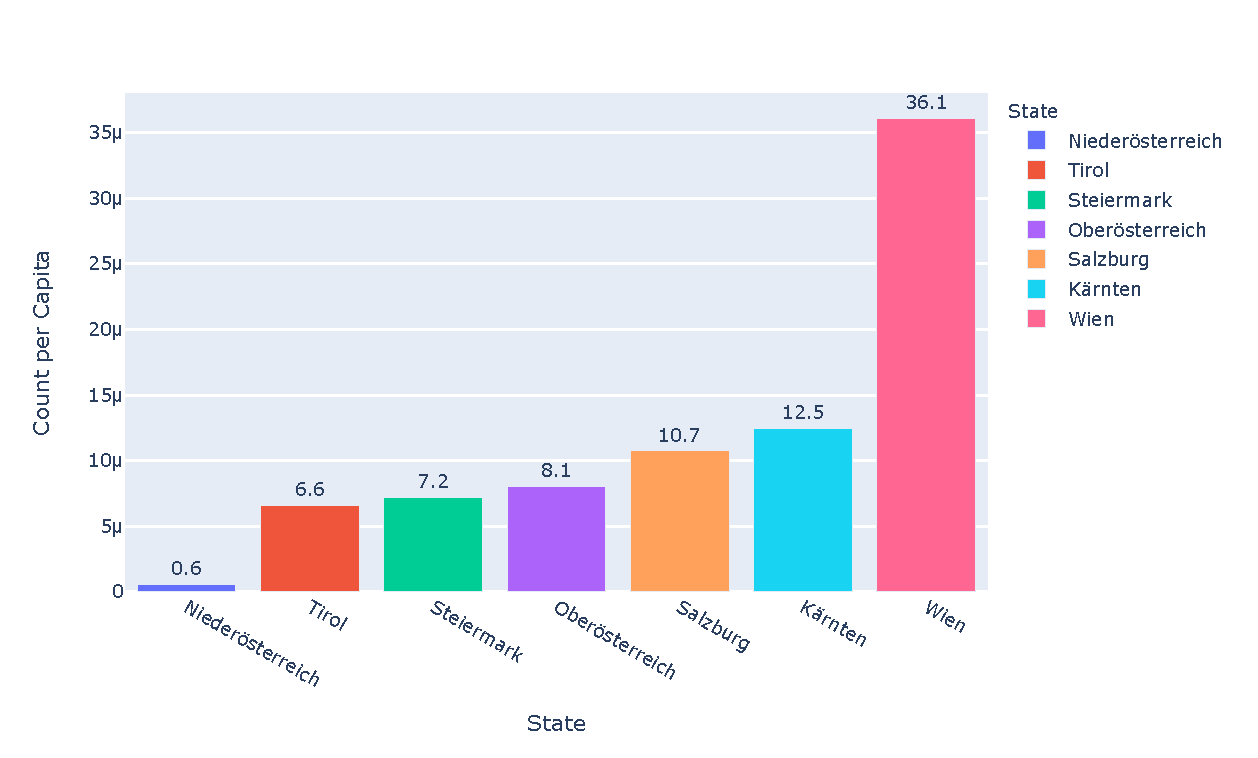
\includegraphics[width=\textwidth]{location-per-capita-bar-chart.pdf}
	\caption{Location per Capita}
	\label{fig:location_per_capita_chart}
\end{figure}

Of the other states, only Carinthia, Styria and Upper Austria manage to pass the 5\% threshold. Tirol and Salzburg are both at around 4\% and Lower Austria is at less than 1\% of all advertisements. Vorarlberg and Burgenland do not even have one job advertisement listed.

To further analyse this, we used the population data included in the Austria Cities Database \cite{austria_cities_database} we used for data cleaning and calculated the per capita numbers for each state as seen in \autoref{fig:location_per_capita_chart}. The vast majority of advertisements were still for positions in Vienna with almost 3 times as many as the per capita in Carinthia. The relative order of Tirol, Salzburg and Carinthia stayed the same while both Styria and Upper Austria dropped by two places, respectively. Most surprising of all is still Lower Austria with the lowest per capita of all states with more than 0 advertisement. This is especially surprising since Lower Austria encloses Vienna. The close vicinity to Vienna is probably a decisive reason for this dramatic disparity.

Let us now look at the average salary. According to our collected data, the total average salary for information security jobs in Austria is 3715.66 € per month. When looking at the numbers per state, we can see the average salary ranging from 3079 € in Tirol to 4160 € in Salzburg. Given this range we already see a surprisingly huge difference of 1081 € between two the neighbouring states Tirol and Salzburg. The average salary in Vienna is closest to the country's total average with only a 1\% deviation. For Lower Austria as well as Burgenland and Vorarlberg we could not extract any salary data.

\begin{figure}[H]
	\centering
  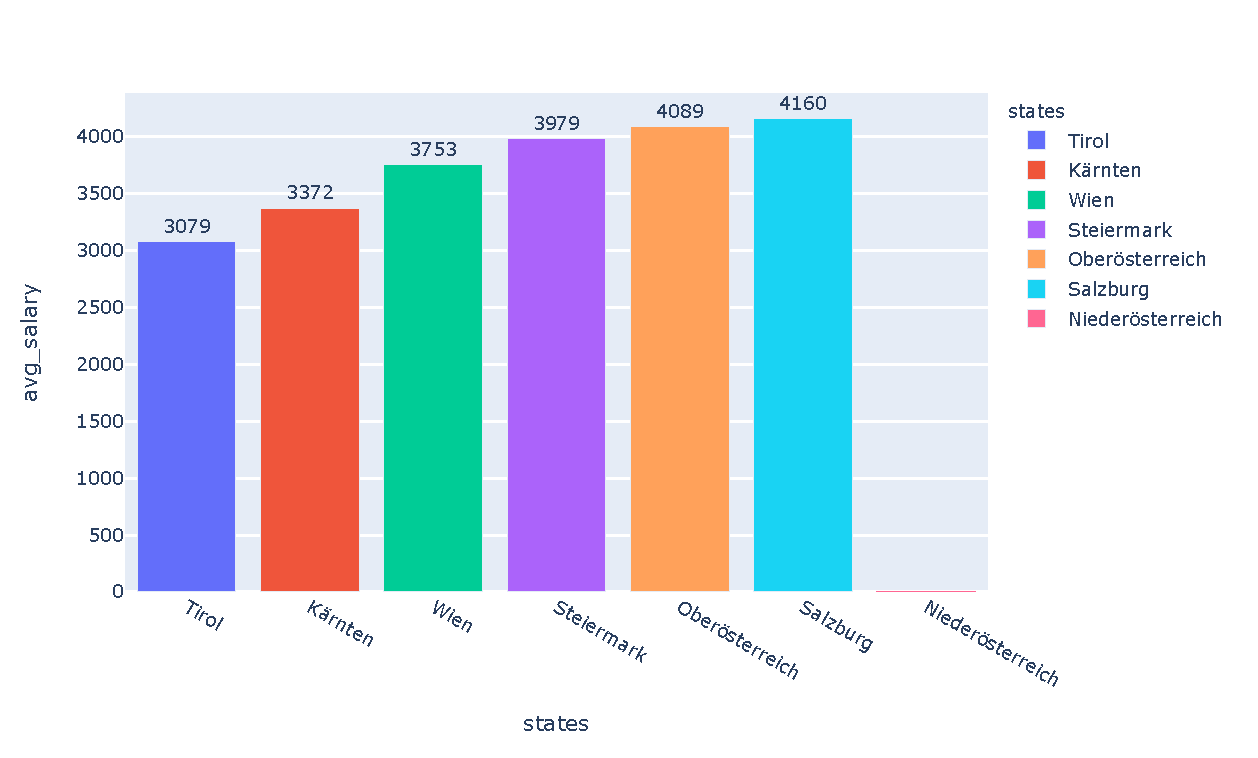
\includegraphics[width=\textwidth]{average-salary-bar-chart.pdf}
	\caption{Salary}
	\label{fig:salary_chart}
\end{figure}

Lastly we will analyse the certifications we extracted. Among the most popularly required certifications are CISM, CISA, ITIL, CISSP and ISO/IEC~27001 (refer to \autoref{tab:certifications} for the certifications' descriptions) with all being specified in at least 20\% of advertisements. With 26\% of jobs advertisements mentioning ISO/IEC~27001, it is by far the most requested requirement. In total, 62 out of 121 job advertisements -- 51 \% --, specify at least one certification as a requirement.

\begin{figure}[H]
	\centering
  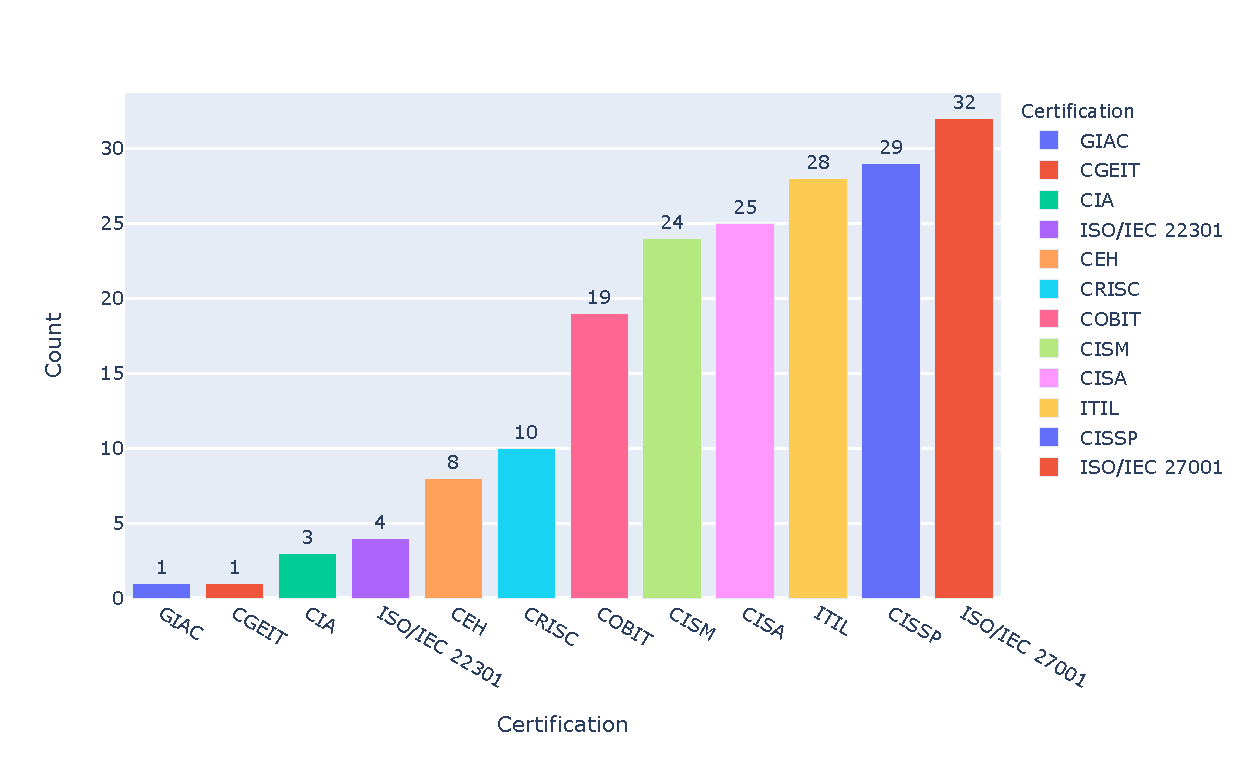
\includegraphics[width=\textwidth]{certifications-bar-chart.pdf}
	\caption{Certifications}
	\label{fig:certifications_chart}
\end{figure}

\section{Conclusion}
\label{sec:conclusion}

In this paper we compared multiple scraping tools highlighting their strong and weak points. Using our chosen scraping tool, we subsequently developed a program for scraping data from three job search sites and used the gathered data to form an overview of the information security job landscape in Austria. Finally, we presented our findings made by analysing the gathered data. These findings can hopefully be used to inform new decisions on what should be taught in universities with regards to information security in order to teach students the skills necessary to succeed in the information security sector.

Some more data points which were not possible to be extracted in this survey could be implemented in a future revision. This includes, for example, the occupational field, which in our survey was not included since only one of the three websites provided this information. Another example includes required knowledge of technologies, which would require a more sophisticated data extraction method than the one used in this survey.

Of course, in order to reduce the chance of outliers skewing the results, the survey could be conducted again within a longer time span and if possible with additional job search websites.

\newpage
\printbibliography

\end{document}
